\chapter{Translation Assistance by Translation of L1 Fragments in an L2 Context}
\title{Translation of L1 Fragments in an L2 Context}
\label{chap:colibritapilot}

In this chapter we present new research in translation assistance. We
describe a pilot system capable of translating native language (L1)
fragments to foreign language (L2) fragments in an L2
context. Practical applications of this research can be framed in
the context of second language learning.  The type of translation
assistance system under investigation here encourages language
learners to write in their target language while allowing them to
fall back to their native language in case the correct word or
expression is not known. These code switches are subsequently
translated to L2 given the L2 context.  We study the
feasibility of exploiting cross-lingual context to obtain
high-quality translation suggestions that improve over statistical
language modelling and word-sense disambiguation baselines. A
classification-based approach is presented that is indeed found to
improve significantly over these baselines by making use of a
contextual window spanning a small number of neighbouring words.

\nobibliography*
\textsc{This chapter is based on: }
\begin{NoHyper}\bibentry{COLIBRITAPILOT}\end{NoHyper}



\section{Introduction}

Whereas machine translation generally concerns the translation of
whole sentences or texts from one language to the other, this study
focusses on the translation of native language (henceforth L1) words
and phrases, i.e. smaller fragments, in a foreign language (L2)
context. Despite the major efforts and improvements, automatic
translation does not yet rival human-level quality. Vexing issues are
morphology, word-order change and long-distance dependencies. Although
there is a morpho-syntactic component in this research, our
scope is more constrained; its focus is on the faithful preservation
of meaning from L1 to L2, akin to the role of the translation model in
Statistical Machine Translation (SMT).
%Our problem is therefore
%more localised compared to SMT and thus evades some of the additional
%complexities in the syntactic domain.

The cross-lingual context in our research question may at first seem
artificial, but its design explicitly aims at applications related to
computer-aided language learning \citep{CALL2,CALL} and computer-aided
translation \citep{CAT}. Currently, language learners need to refer to a
bilingual dictionary when in doubt about a translation of a word or phrase.
Yet, this problem arises in a context, not in isolation; the learner may have
already translated successfully a part of the text into L2 leading up to the
problematic word or phrase. Dictionaries are not the best source to look up
context; they may contain example usages, but remain biased towards single
words or short expressions.

The proposed application allows code switching and produces context-sensitive
suggestions as writing progresses. In this research we test the feasibility of
the foundation of this idea.The following examples serve to illustrate the idea
and demonstrate what output the proposed translation assistance system would
ideally produce. The parts in bold correspond to respectively the inserted
fragment and the system translation.

\begin{itemize}
  \item
    Input (L1=English,L2=Spanish): \emph{“Hoy vamos a \textbf{the swimming
    pool}.”} \\
    Desired output: \emph{“Hoy vamos a \textbf{la piscina}.”}
  \item
    Input (L1-English, L2=German): \emph{“Das wetter ist wirklich
    \textbf{abominable}.”} \\
    Desired output: \emph{“Das wetter ist wirklich \textbf{ekelhaft}.”}
  \item
    Input (L1=French,L2=English): \emph{“I \textbf{rentre à la maison} because
    I am tired.”} \\
    Desired output: \emph{“I \textbf{return home} because I am tired.”}
  \item
    Input (L1=Dutch, L2=English): \emph{“Workers are facing a massive \textbf{aanval
    op} their employment and social rights.”} \\
    Desired output: \emph{“Workers are facing a massive \textbf{attack on}
    their employment and social rights.”}
\end{itemize}


The main research question in this research is how to disambiguate an L1 word
or phrase to its L2 translation based on an L2 context, and whether such
cross-lingual contextual approaches provide added value compared to baseline
models that are not context informed or compared to standard language models.



\section{Data preparation}

Preparing the data to build training and test data for our intended
translation assistance system is not trivial, as the type of
interactive translation assistant we aim to develop does not exist yet. We
need to generate training and test data that realistically emulates
the task. We start with a parallel corpus that is tokenised for both
L1 and L2. No further linguistic processing such as part-of-speech
tagging or lemmatisation takes place in our experiments; adding this
remains open for future research.
% and may likely lead to further
%improvements in the results.

The parallel corpus is randomly sampled into two large and
equally-sized parts. One is the basis for the training set, and the
other is the basis for the test set. The reason for such a large test
split shall become apparent soon.

From each of the splits ($S$), a phrase-translation table is constructed
automatically in an unsupervised fashion. This is done using the scripts
provided by the Statistical Machine Translation system Moses \citep{MOSES}. It
invokes GIZA++ \citep{GIZA} to establish statistical word alignments based on
the IBM Models and subsequently extracts phrases using the
\texttt{grow-diag-final} algorithm \citep{OchNey2003}. The result, independent
for each set, will be a phrase-translation table ($T$) that maps phrases in L1
to L2. For each phrase-pair ($f_s,f_t$) this phrase-translation table holds the computed
translation probabilities $P(f_s|f_t)$ and $P(f_t|f_s)$.

Given these phrase-translation tables, we can now extract both training data
and test data using the algorithm in Figure~\ref{fig:algo}.  In our discourse, the source language ($s$) corresponds to L1, the
fallback language used for by the end-user for inserting fragments, whilst the
target language ($t$) is L2.

\begin{figure}[t]
\begin{framed}
\begin{enumerate}
%\footnotesize
\item using phrase-translation table $T$ and parallel corpus split $S$
\item \textbf{for} each aligned sentence pair $({sentence}_s \in
  S_s,{sentence}_t \in S_t)$ in the parallel corpus split ($S_s$,$S_t$):
\item \hspace{5mm}\textbf{for} each fragment $(f_s \in {sentence}_s, f_t \in
  {sentence}_t)$ where $(f_s, f_t) \in T$:
\item \hspace{10mm}\textbf{if} $P(f_s|f_t) \cdot P(f_t|f_s) \geq \lambda_1$
  \textbf{and} $P(f_s|f_t) \cdot P(f_t|f_s) \geq
  \lambda_2 \cdot P(f_s|f_{strongest\_t}) \cdot  P(f_{strongest\_t}|f_s)$:
\item \hspace{15mm}Output a pair $({sentence}_t',{sentence}_t)$ where
  ${sentence}_t'$ is a copy of $t$ but with
  fragment $f_t$ substituted by $f_s$, i.e. the introduction of an L1 word or phrase in an L2 sentence.
\end{enumerate}
\end{framed}
\caption{Algorithm for extracting training and test data on the basis of a
phrase-translation table ($T$) and subset/split from a parallel corpus ($S$).
The indentation indicates the nesting.}
\label{fig:algo}
\end{figure}

Step 4 is effectively a filter: two thresholds can be configured to discard
weak alignments, i.e. those with low probabilities, from the phrase-translation
table so that only strong couplings make it into the generated set. The
parameter $\lambda_1$ adds a constraint based on the product of the two
conditional probabilities $(P(f_t|f_s) \cdot P(f_s|f_t))$, and sets a threshold
that has to be surpassed.  A second parameter $\lambda_2$  further limits the
considered phrase pairs $(f_s,f_t)$ to have the product of their conditional
probabilities not deviate more than a fraction $\lambda_2$ from the joint
probability for the strongest possible pairing for $f_s$, the source fragment.
In Figure~{fig:algo}, $f_{strongest\_t}$ corresponds to the best scoring
translation for a given source fragment $f_s$. This metric thus effectively
prunes weaker alternative translations in the phrase-translation table from
being considered if there is a much stronger candidate. Nevertheless, it has to
be noted that even with $\lambda_1$ and $\lambda_2$, the test set will include
a certain amount of errors. This is due to the nature of the unsupervised
method with which the phrase-translation table is constructed. For our purposes
however, the test set suffices to test our hypothesis.

In our experiments, we choose fixed values for these parameters, by
manual inspection and judgement of the output. The $\lambda_1$
parameter was set to $0.01$ and $\lambda_2$ to $0.8$.  Whilst other
thresholds may possibly produce cleaner sets, this is hard to evaluate
as finding optimal values causes a prohibitive increase in complexity
of the search space, and again this is not necessary to test our hypothesis.

The output of the algorithm in Figure~\ref{fig:algo} is a modified set of sentence pairs
$({sentence}_t',{sentence}_t)$, in which the same sentence pair may be used multiple times
with different L1 substitutions for different fragments.
%A single L2
%sentence $t$ may thus occur in multiple sentence pairs.
The final
test set is created by randomly sampling the desired number of test
instances.

Note that the training set and test set are constructed on their own
respective and independently generated phrase-translation tables. This
ensures complete independence of training and test data. Generating
test data using the same phrase-translation table as the training data
would introduce a bias. The fact that a phrase-translation table needs
to be constructed for the test data is also the reason that the
parallel corpus split from which the test data is derived has to be
large enough, ensuring better quality.

We concede that our current way of testing is a mere approximation of the real-world scenario. An ideal test corpus
would consist of L2 sentences with L1 fallback as crafted by L2 language learners with an L1 background. However, such
corpora do not exist yet at the time of this research. Nevertheless, we hope to show that our automated way of test set
generation is sufficient to test the feasibility of our core hypothesis that L1 fragments can be translated to L2 using
L2 context information.

\section{System}

We develop a classifier-based system composed of so-called ``classifier
experts''. Numerous classifiers are trained and each is an expert in
translating a single word or phrase. In other words, for each word type or
phrase type that occurs as a fragment in the training set, and which does not
map to just a single translation, a classifier is trained.  The classifier maps
the L1 word or phrase in its L2 context to its L2 translation. Words or phrases
that always map to a single translation are stored in a simple mapping table,
as a classifier would have no added value in such cases. The classifiers use
the IB1 algorithm \citep{IB1} as implemented in TiMBL
\citep{TIMBL}.\footnote{\url{https://languagemachines.github.io/timbl}} IB1 implements
$k$-nearest neighbour classification. The choice for this algorithm is
motivated by the fact that it handles multiple classes with ease, but first and
foremost because it has been successfully employed for word sense
disambiguation in other studies \citep{Hoste+02,GAMBL}, in particular in
cross-lingual word sense disambiguation as seen in Chapter~\ref{chap:clwsd}. It has
also been used in machine translation studies in which local source context is
used to classify source phrases into target phrases, rather than looking them
up in a phrase table \citep{Stroppa+07,Haque+11}. The idea of local phrase
selection with a discriminative machine learning classifier using additional
local (source-language) context was introduced in parallel to \cite{Stroppa+07} by \cite{Carpuat+07} and
\cite{Gimenez+07}; cf. \cite{Haque+11} for an overview of more recent methods.

The feature vector for the classifiers represents a local context of
neighbouring words, and optionally also global context keywords in a
binary-valued bag-of-words configuration. The local context consists
of an $X$ number of L2 words to the left of the L1 fragment, and $Y$
words to the right.

When presented with test data, in which the L1 fragment is explicitly marked,
we first check whether there is ambiguity for this L1 fragment and if a direct
translation is available in our simple mapping table. If so, we are done
quickly and need not rely on context information. If not, we check for the
presence of a classifier expert for the offered L1 fragment; only then we can
proceed by extracting the desired number of L2 local context words to the
immediate left and right of this fragment and adding those to the feature
vector. The classifier will return a probability distribution of the most likely
translations given the context and we can replace the L1 fragment with the
highest scoring L2 translation and present it back to the user.

In addition to local context features, we also experimented with
global context features. These are a set of L2 contextual keywords for
each L1 word/phrase and its L2 translation occurring in the same
sentence, not necessarily in the immediate neighbourhood of the L1
word/phrase. The keywords are selected to be indicative for a specific
translation. We used the method of extraction by \cite{NgL96}, as we have seen in Chapter~\ref{chap:clwsd}, and
encoded all keywords in a binary bag of words model. The experiments
however showed that inclusion of such keywords did not make any
noticeable impact on any of the results, so we restrict ourselves to
mentioning this negative result.

%<paraphrase from earlier paper>
%In addition to this, {\em global context}\/ features may be extracted; these are
%a set of L2 keywords per L1 word/phrase and its L2 translation. The keywords
%have to be found occurring above certain occurrence thresholds at arbitrary
%positions in the same sentence. The global context features are represented as
%a binary bag-of-words model in which the presence of each of the keywords that
%may be indicative for a given mapping of the focus word/phrase to a translation
%is represented by a boolean value. Such a set of keywords is constructed
%independently for each classifier. For some classifiers no keywords
%may be found.

%The method used to extract these keywords ($k$) is proposed by
%\newcitep{NgL96}.
%Assume we have a fragment $f$, more precisely, an
%L1 word or phrase.  We also have one of its aligned L2 translations
%$s$. We can now estimate $P(s|k)$, the probability of translation $s$,
%given an L2 keyword $k$. Let $N_{s,k_{local}.}$ be the number of
%occurrences of a possible context word $k$ pertaining to a particular
%combination of L1 fragment and L2 translation $s$. Let $N_{k_{local}}$
%be the number of occurrences of a possible local context keyword $k$
%pertaining to a particular L1 fragment but regardless of its
%translation. If we also take into account the frequency of a possible
%keyword $k$ in the complete training corpus ($N_{k_{corpus}}$), we
%get:

%\begin{equation}
%P(s|k) = \frac{N_{s,k_{local}}}{N_{k_{local}}}(\frac{1}{N_{k_{corpus}}})
%\end{equation}

%\newcitep{Hoste+02} select a keyword $k$ for inclusion in the bag-of-words
%representation if that keyword occurs more than $T_1$ times in that translation
%$s$, and if $P(s|k) \ge T_2$. Both $T_1$ and $T_2$ are predefined thresholds,
%which by default were set to $3$ and $0.001$ respectively. We adopted these same
%values.

%The selection of bag-of-word features is computed prior to the
%extraction of the training instances, as this information is a prerequisite for
%the successful generation of both training and test instances.
%</paraphrase from earlier paper>

Our full system, including the scripts for data preparation, training, and
evaluation, is implemented in Python and freely available as open-source from
\url{https://github.com/proycon/colibrita/} . Version tag \texttt{v0.2.1} is
representative for the version used in this research.


\subsection{Language Model}

%This led us to
We also implement a statistical language model as an optional component of our
classifier-based system and also as a baseline to compare our system to.  The
language model is a trigram-based back-off language model with Kneser-Ney
smoothing, computed using SRILM \citep{SRILM} and trained on the same training
data as the translation model. No additional external data was brought in, to
keep the comparison fair.

For any given hypothesis $H$, results from the L1 to L2 classifier are combined with
results from the L2 language model. We do so by normalising the class
probability from the classifier ($score_T(H)$), which is our translation model, and the language model
($score_{lm}(H)$), in such a way that the highest classifier score for
the alternatives under consideration is always $1.0$, and the highest
language model score of the sentence is always $1.0$. Take $score_T(H)$
and $score_{lm}(H)$ to be log probabilities, the search for the best (most
probable) translation hypothesis $\hat{H}$ can then be expressed as:

\begin{equation}
  \hat{H} = \arg\max_H (score_T(H) + score_{lm}(H))
  \label{eq:LM}
\end{equation}

If desired, the search can be parametrised with variables $\lambda_3$ and
$\lambda_4$, representing the weights we want to attach to the classifier-based
translation model and the language model, respectively. In the current study we
simply left both weights set to one, thereby assigning equal importance to
translation model and language model.

%\begin{equation}
%  \arg\max_B = \lambda_3 score_T + \lambda_4 score_{lm}
%\end{equation}

% maar deze equation is dan eigenlijk een beetje overbodig...
%da's waar,  weggehaald, scheelt weer ruimte

\section{Evaluation}

Several automated metrics exist for the evaluation of L2 system
output against the L2 reference output in the test set. We first
measure absolute accuracy by simply counting all output fragments that
exactly match the reference fragments, as a fraction of the total
amount of fragments. This measure may be too strict, so we add a more
flexible \emph{word accuracy} measure which takes into account partial
matches at the word level. If output $o$ is a subset of reference $r$
then a score of $\frac{|o|}{|r|}$ is assigned for that sentence
pair. If instead, $r$ is a subset of $o$, then a score of
$\frac{|r|}{|o|}$ will be assigned. A perfect match will result
in a score of $1$ whereas a complete lack of overlap will be
scored $0$. The word accuracy for the entire set is then computed by
taking the sum of the word accuracies per sentence pair, divided by
the total number of sentence pairs.

We also compute a recall metric that measures the number of fragments that the
system provided a translation for as a fraction of the total number of
fragments in the input, regardless of whether the fragment is translated
correctly or not. The system may skip fragments for which it can find no
solution at all.

In addition to these, the system's output can be compared against the
L2 reference translation(s) using established Machine Translation
evaluation metrics.  We report on BLEU, NIST, METEOR, and word error
rate metrics WER and PER.  These scores should generally be much
better than the typical MT system performances as only local changes
are made to otherwise ``perfect'' L2 sentences.

\section{Baselines}

A context-insensitive yet informed baseline was constructed to assess
the impact of L2 context information in translating L1 fragments. The
baseline selects the most probable L1 fragment per L2 fragment
according to the phrase-translation table. This baseline, henceforth
referred to as the 'most likely fragment' baseline (MLF) is analogous
to the 'most frequent sense'-baseline common in evaluating WSD
systems.

A second baseline was constructed by weighing the probabilities from
the translation table directly with the L2 language model described
earlier. It adds a LM component to the MLF baseline. This LM baseline
allows the comparison of classification through L1 fragments in an L2
context, with a more traditional L2 context modelling (i.e. target
language modelling) which is also customary in MT decoders. Computing
this baseline is done in the same fashion as previously illustrated in
Equation~\ref{eq:LM}, where $score_T$ then represents the normalised
$p(t|s)$ score from the phrase-translation table rather than the class
probability from the classifier.

\section{Experiments \& Results}

The data for our experiments were drawn from the Europarl parallel corpus
\citep{EUROPARL} from which we extracted two sets of $200,000$ sentence
pairs each for several language pairs. These were used to form the
training and test sets. The final test sets are a randomly sampled
$5,000$ sentence pairs from the $200,000$-sentence test split for each
language pair.

All input and output data for the experiments in this section are publicly available\footnote{Obtain all experimental input data
with corresponding output and evaluation results from \url{https://lst.science.ru.nl/~proycon/colibrita-acl2014-data.zip}}.

Let us first zoom in to convey a sense of scale on a specific
language pair. The actual Europarl training set we generate for
English (L1) to Spanish (L2), i.e. English fallback in a Spanish
context, consists of $5,608,015$ sentence pairs. This number is much
larger than the $200,000$ we mentioned before because single sentence
pairs may be reused multiple times with different marked fragments.
From this training set of sentence pairs over $100,000$ classifier
experts are derived. The eleven largest classifiers are shown in
Table~\ref{tab:topexperts}, along with the number of training
instances per classifier. The full table would reveal a Zipfian
distribution.

\begin{table}[hbt]
\footnotesize
\noindent\makebox[\textwidth][c]{%
\begin{tabular}{lll}
\hline
Fragment & Training instances & Translations \\
\hline
the & 256,772 & la, el, los, las  \\
of &   139,273 & de, del \\
and &  128,074 & y, de, e \\
to &   66,565 & a, para, que, de \\
a &  54,306 & un, una \\
is &  40,511 & es, está, se \\
for & 34,054 & para, de, por \\
this & 29,691 & este, esta, esto \\
European & 26,543 & \pbox{3cm}{Europea, Europeo \\ Europeas, Europeos} \\
on & 23,147 & sobre, en \\
of the & 22,361 & de la, de los\\
\hline
\end{tabular}}
\caption{The top eleven classifier experts for English to Spanish. The eleventh
entry is included as an example of a common phrasal fragment.}
\label{tab:topexperts}
\end{table}

Among the classifier experts are only words and phrases that are
ambiguous and may thus map to multiple translations. This implies that
such words and phrases must have occurred at least twice in the
corpus, though this threshold is made configurable and could have been
set higher to limit the number of classifiers. The remaining $246,380$
unambiguous mappings are stored in a separate mapping table.

For the classifier-based system, we tested various different feature
vector configurations. The first experiment, of which the results are
shown in Figure~\ref{fig:context}, sets a fixed and symmetric local
context size across all classifiers, and tests three context
widths. Here we observe that a context width of one yields the best
results. The BLEU scores, not included in the figure but shown in
Table~\ref{tab:results}, show a similar trend. This trend holds for
all the MT metrics.

%It is also worth noting that as
%expected, all metrics correlate as they all measure essentially the
%same thing; overlap between the system output and the reference
%translation in the test set, but in different ways and focussing on
%different aspects.

Table~\ref{tab:results} shows the results for English to Spanish in
more detail and adds a comparison with the two baseline systems. The various
\texttt{lXrY} configurations use the same feature vector setup for all classifier
experts. Here $X$ indicates the left context size and $Y$ the right context
size.
%Each of these configurations uses the same feature
%vector setup across all classifier experts
The \texttt{auto} configuration
does not uniformly apply the same feature vector setup to all classifier
experts but instead seeks to find the optimal setup per
classifier expert. This shall be further discussed in
Section~\ref{sec:optim}.

\begin{figure}[t]
\centering
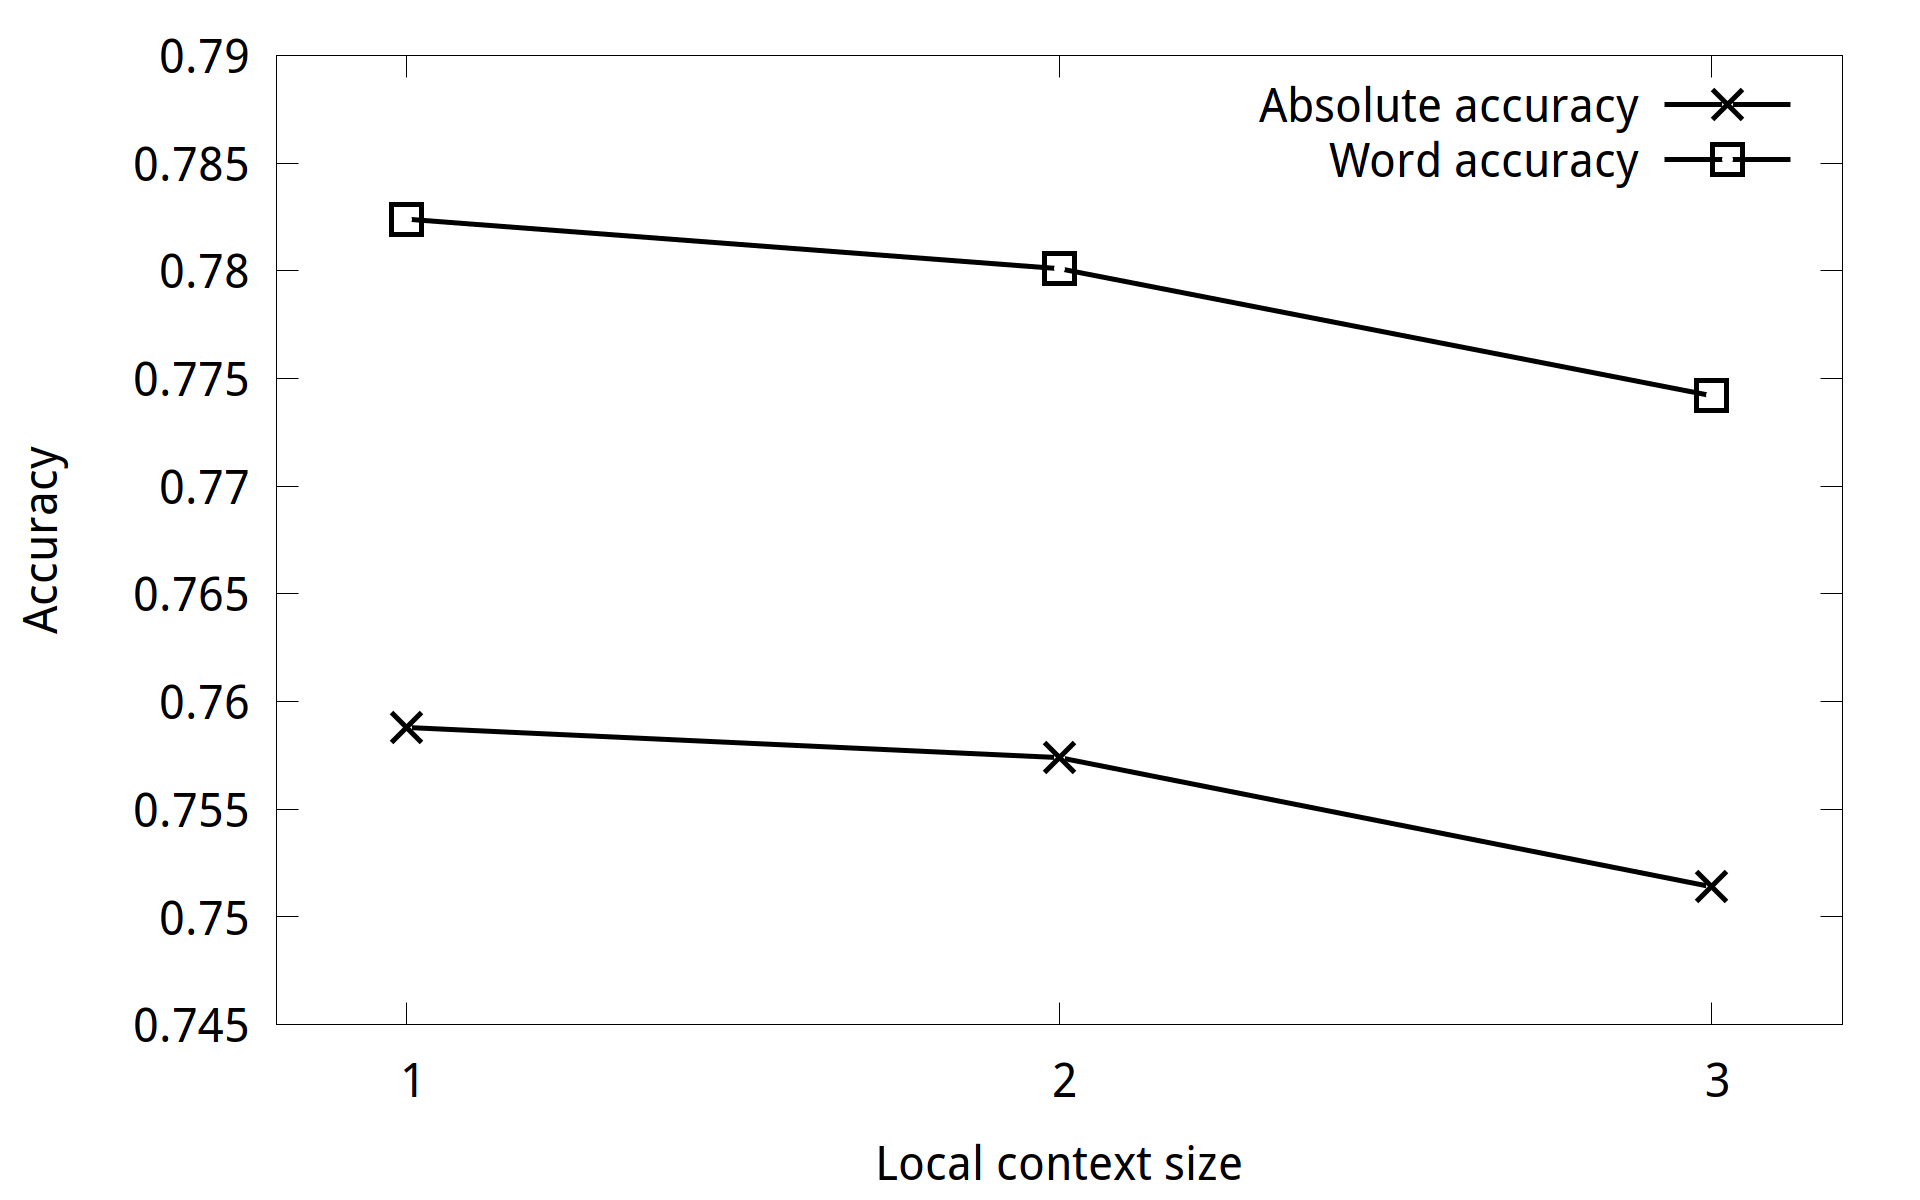
\includegraphics[width=12cm]{colibritapilot-context.png}
\caption{Accuracy for different local context sizes, Europarl English to Spanish.}
\label{fig:context}
\end{figure}



\begin{center}
\begin{table*}[bt]
\footnotesize{
\noindent\makebox[\textwidth][c]{%
\begin{tabular}{llllllll}
\hline
Configuration & Accuracy & Word Accuracy & BLEU & METEOR & NIST & WER & PER \\
\hline
MLF baseline & 0.6164 & 0.6662 & 0.972 & 0.9705 & 17.0784 & 1.4465 & 1.4209 \\
LM baseline & 0.7158 & 0.7434 & 0.9785 & 0.9739 & 17.1573 & 1.1735 & 1.1574 \\
\hline
l1r1 & 0.7588 & 0.7824  & 0.9801 & 0.9747 & 17.1550 & 1.1625 & 1.1444 \\
l2r2 & 0.7574 & 0.7801 & 0.9800 & 0.9746 & 17.1550 & 1.1750 & 1.1569 \\
l3r3 & 0.7514 & 0.7742 & 0.9796 & 0.9744 & 17.1445 & 1.1946 & 1.1780 \\
\hline
l1r1$+$LM & \textbf{0.7810} & \textbf{0.7973} & \textbf{0.9816} &
\textbf{0.9754} & \textbf{17.1685} & \textbf{1.0946} & \textbf{1.077} \\
\hline
%l1r1k & 0.7586 & 0.7823 & 0.9801 & 0.9747 & 17.1548 & 1.1630 & 1.1449 \\
%\hline
auto & 0.7626 & 0.7850 & 0.9803 & 0.9748 & 17.1544 & 1.1594 & 1.1424 \\
auto$+$LM & 0.7796 & 0.7966 & 0.9815 & 0.9754 & 17.1664 & 1.1021 & 1.0845 \\
\hline
l1r0 & 0.6924 & 0.7223 & 0.9757 & 0.9723 & 17.1087 & 1.3415 & 1.3249\\
l2r0 & 0.6960 & 0.7245 & 0.9759 & 0.9724 & 17.1091 & 1.3364 & 1.3193\\
l2r1 & 0.7624 & 0.7849 & 0.9803 & 0.9748 & 17.1558 & 1.1554 & 1.1378\\
\hline
\end{tabular}}
}
\caption{Europarl results for English to Spanish (i.e English fallback in
Spanish context). Recall $ = 0.9422$.}
\label{tab:results}
\end{table*}
\end{center}


As expected, the LM baseline substantially outperforms the
context-insensitive MLF baseline. Second, our classifier approach
attains a substantially higher accuracy than the LM baseline. Third,
we observe that adding the language model to our classifier leads to
another significant gain (configuration \texttt{l1r1$+$LM} in the
results in Table~\ref{tab:results}).  It appears that the classifier
approach and the L2 language model are able to complement each other.

Statistical significance on the BLEU scores was tested using pairwise bootstrap
sampling \citep{KoehnStatSig}.  All significance tests were performed with
$5,000$ iterations.  We compared the outcomes of several key configurations. We
first tested \texttt{l1r1} against both baselines; both differences are
significant at $p<0.01$ for both. The same significance level was found when
comparing \texttt{l1r1$+$LM} against \texttt{l1r1}, \texttt{auto$+$LM} against
\texttt{auto}, as well as the LM baseline against the MLF baseline. Automatic
feature selection \texttt{auto} was found to perform statistically better than
\texttt{l1r1}, but only at $p<0.05$. Conclusions with regard to context width
may have to be tempered somewhat, as the performance of the \texttt{l1r1}
configuration was found to not be significantly better than that of the
\texttt{l2r2} configuration. However, \texttt{l1r1} performs significantly
better than \texttt{l3r3} at $p<0.01$, and \texttt{l2r2} performs significantly
better than \texttt{l3r3} at $p<0.01$.

% ~/mtevalscripts/paired_bootstrap_v13a/paired_bootstrap_resampling_bleu_v13a.pl pb_l1r1.statsfile pb_baseline.statsfile 5000 0.05
%System 1 BLEU better: 5000 / 5000 = 1 -- BLEU SIGNIFICANT at p = 0.05                                                                               │···················

%~/mtevalscripts/paired_bootstrap_v13a/paired_bootstrap_resampling_bleu_v13a.pl pb_l1r1lm.statsfile pb_l1r1.statsfile 5000 0.05
% System 1 BLEU better: 5000 / 5000 = 1 -- BLEU SIGNIFICANT at p = 0.05

%~/mtevalscripts/paired_bootstrap_v13a/paired_bootstrap_resampling_bleu_v13a.pl pb_lmbaseline.statsfile pb_baseline.statsfile 5000 0.05
% System 1 BLEU better: 5000 / 5000 = 1 -- BLEU SIGNIFICANT at p = 0.05

% ~/mtevalscripts/paired_bootstrap_v13a/paired_bootstrap_resampling_bleu_v13a.pl pb_al5r5k.statsfile pb_l1r1.statsfile 5000 0.05
%System 1 BLEU better: 4818 / 5000 = 0.9636 -- BLEU SIGNIFICANT at p = 0.05

%~/mtevalscripts/paired_bootstrap_v13a/paired_bootstrap_resampling_bleu_v13a.pl pb_al5r5klm.statsfile pb_al5r5k.statsfile 5000 0.05
%System 1 BLEU better: 5000 / 5000 = 1 -- BLEU SIGNIFICANT at p = 0.05

%proycon@scootaloo /scratch/proycon/colibrita/2/europarl200k-en-es$ ~/mtevalscripts/paired_bootstrap_v13a/paired_bootstrap_resampling_bleu_v13a.pl pb_l1r1lm.statsfile pb_al5r5k.statsfile 5000 0.05
%System 1 BLEU better: 5000 / 5000 = 1 -- BLEU SIGNIFICANT at p = 0.05

%~/mtevalscripts/paired_bootstrap_v13a/paired_bootstrap_resampling_bleu_v13a.pl pb_l1r1.statsfile pb_l2r2.statsfile 5000 0.05    master 16:05:04
%System 1 BLEU better: 4159 / 5000 = 0.8318

%l1 over l3
%System 1 BLEU better: 4994 / 5000 = 0.9988 -- BLEU SIGNIFICANT at p = 0.05

%l2 over l3
%System 1 BLEU better: 4998 / 5000 = 0.9996 -- BLEU SIGNIFICANT at p = 0.05



In Table~\ref{tab:example} we present some illustrative examples from
the English $\rightarrow$ Spanish Europarl data. We show the difference
between the most-likely-fragment baseline and our system.

\begin{table*}[htb]
\begin{framed}
\footnotesize
\textbf{Input:} Mientras no haya prueba en contrario , la financiación de partidos políticos \textbf{European} sólo se justifica , incluso después del tratado de Niza , desde el momento en que concurra a la expresión del sufragio universal , que es la única definición aceptable de un partido político . \\
\textbf{MLF baseline:} Mientras no haya prueba en contrario , la financiación de partidos políticos \textbf{Europea} sólo se justifica , incluso después del tratado de Niza , desde el momento en que concurra a la expresión del sufragio universal , que es la única definición aceptable de un partido político . \\
\textbf{l1r1:} Mientras no haya prueba en contrario , la financiación de partidos políticos \textbf{europeos} sólo se justifica , incluso después del tratado de Niza , desde el momento en que concurra a la expresión del sufragio universal , que es la única definición aceptable de un partido político .\\
\line(1,0){250} \\
\textbf{Input:} Esta Directiva es nuestra oportunidad \textbf{to} marcar una verdadera
diferencia , reduciendo la trágica pérdida de vidas en nuestras carreteras . \\
\textbf{MLF baseline:} Esta Directiva es nuestra oportunidad \textbf{a} marcar una
verdadera diferencia , reduciendo la trágica pérdida de vidas en nuestras
carreteras . \\
\textbf{l1r1:} Esta Directiva es nuestra oportunidad \textbf{para} marcar una
verdadera diferencia , reduciendo la trágica pérdida de vidas en nuestras
carreteras . \\
\line(1,0){250} \\
\textbf{Input:} Es la \textbf{last} vez que me dirijo a esta Cámara . \\
\textbf{MLF baseline:} Es la \textbf{pasado} vez que me dirijo a esta Cámara .\\
\textbf{l1r1:} Es la \textbf{última} vez que me dirijo a esta Cámara .\\
\line(1,0){250} \\
\textbf{Input:} Pero el enfoque actual de la Comisión no puede conducir a una buena
política ya que es tributario del funcionamiento del mercado y de las normas
establecidas por la OMC , el FMI y el Banco Mundial , normas que siguen siendo
desfavorables para los \textbf{developing countries} . \\
\textbf{MLF baseline:} Pero el enfoque actual de la Comisión no puede conducir a
una buena política ya que es tributario del funcionamiento del mercado y de las
normas establecidas por la OMC , el FMI y el Banco Mundial , normas que siguen
siendo desfavorables para los \textbf{los países en desarrollo} . \\
\textbf{l1r1:} Pero el enfoque actual de la Comisión no puede conducir a
una buena política ya que es tributario del funcionamiento del mercado y de las
normas establecidas por la OMC , el FMI y el Banco Mundial , normas que siguen
siendo desfavorables para los \textbf{países en desarrollo} .
\end{framed}
\caption{Some illustrative examples of MLF-baseline output versus system output, in
which system output matches the correct human reference output. The actual fragments
concerned are highlighted in bold. The first example shows our system
correcting for number agreement, the second a correction in selecting the right preposition, and the
third shows that the English word \emph{last} can be translated in different ways, only one of which
is correct in this context. The last example shows a phrasal translation, in
which the determiner was duplicated in the baseline.}
\label{tab:example}
\end{table*}

\begin{table*}[htb]
\begin{framed}
\footnotesize
\textbf{Input:} Sin ese tipo de protección la gente no aprovechará la oportunidad \textbf{to} vivir , viajar y trabajar donde les parezca en la Unión Europea . \\
\textbf{l1r1:} Sin ese tipo de protección la gente no aprovechará la oportunidad \textbf{para} vivir , viajar y trabajar donde les parezca en la Unión Europea . \\
\textbf{l1r1$+$LM:} Sin ese tipo de protección la gente no aprovechará la oportunidad \textbf{de} vivir , viajar y trabajar donde les parezca en la Unión Europea . \\
\line(1,0){250} \\
\textbf{Input:} La Comisión también está acometiendo medidas en el ámbito social y \textbf{educational} con vistas a mejorar la situación de los niños . \\
\textbf{l1r1:} La Comisión también está acometiendo medidas en el ámbito social y \textbf{educativas} con vistas a mejorar la situación de los niños .  \\
\textbf{l1r1$+$LM:} La Comisión también está acometiendo medidas en el ámbito social y \textbf{educativo} con vistas a mejorar la situación de los niños . \\
\end{framed}
\caption{Some examples of l1r1 versus the same configuration enriched
  with a language model.}
%The language model version corresponds with the human reference.}
\label{tab:example2}
\end{table*}


Likewise, Table~\ref{tab:example2} exemplifies small fragments from the
\texttt{l1r1} configuration compared to the same configuration enriched with a
language model. We observe in this data that the language model often has the
added power to choose a correct translation that is not the first prediction of
the classifier, but one of the weaker alternatives that nevertheless fits
better.  Though the classifier generally works best in the \texttt{l1r1}
configuration, i.e. with context size one, the trigram-based language model
allows further left-context information to be incorporated that influences the
weights of the classifier output, successfully forcing the system to select
alternatives. This combination of a classifier with context size one and
trigram-based language model proves to be most effective and reaches the best
results so far. We have not conducted experiments with language
models of other orders.

%We initially
%expected the \textbf{auto$+$LM} to obtain better results than
%\textbf{l1r1$+$LM}. However, the complementary effect of classifier
%and language model becomes less pronounced as more context is added to
%the former, taking much of the added value of a language model away.

%We find that the inclusion of global context keywords (the $l1r1k$
%configuration) has no noticeable impact, and this trend holds when
%different language pairs are tested. In one of our English to Dutch
%Europarl sets for example, we find that only $41$ out of $5,000$ test
%sentence pairs trigger a keyword match during testing.  During
%training, keywords were found for $9,910$ out of $112,653$
%classifiers.  The virtually absent impact of global context keywords
%is also in agreement with findings from \newcitep{WSD2}; the trend
%seems to be that simplicity in feature selection pays off and holds
%for all language pairs we tested.

\FloatBarrier

\subsection{Context optimisation}
\label{sec:optim}

It has been argued that classifier experts in a word sense disambiguation
ensemble should be individually optimised \citep{GAMBL}. This we have also shown
in Chapter~\ref{chap:clwsd}, where we find a positive impact when conducting
feature selection per classifier. This intuitively makes sense; a context of
one may seem to be better than any other when uniformly applied to all
classifier experts, but it may well be that certain classifiers benefit from
different feature selections.  We therefore proceed with this line of
investigation as well.

Automatic configuration selection was done by performing leave-one-out
testing (for small number of instances) or 10-fold-cross validation
(for larger number of instances, $n \geq 20$) on the training data per
classifier expert. Various configurations were tested. Per classifier
expert, the best scoring configuration was selected, referred to as
the \texttt{auto} configuration in Table~\ref{tab:results}. The
\texttt{auto} configuration improves results over the uniformly
applied feature selection.  However, if we enable the language model
as we do in the \texttt{auto$+$LM} configuration we do not notice an
improvement over \texttt{l1r1$+$LM}, surprisingly. We suspect the lack
of impact here can be explained by the trigram-based Language Model
having less added value when the (left) context size of the classifier
is two or three; they are now less complementary.

% wat kun je hier meer over zeggen? kun je het verklaren?
% - ik heb een vermoeden, nu hierboven uitgelegd.
%  eventueel zou ik nog experimenten met l2r2LM en l3r3LM kunnen draaien om dit
%  misschien echt hard te kunnen maken.

Table~\ref{tab:autoconf} lists what context sizes have been chosen in the
automatic feature selection. A context size of one prevails in the vast majority of
cases, which is not surprising considering the good results we have already
seen with this configuration.

% hier dan wel iets meer over zeggen, anders mag de lezer raden waarom
% er aandacht en een tabel aan wordt besteed.
% - done, beetje toegevoegd.

\begin{table}[htb]
%\footnotesize
\noindent\makebox[\textwidth][c]{%
\begin{tabular}{rl}
\hline
$66.5\%$ & l1r1\\
$19.9\%$ & l2r2\\
$7.7\%$ & l3r3\\
$3.5\%$ & l4r4\\
$2.4\%$ & l5r5\\
\hline
\end{tabular}}
\caption{Frequency of automatically selected configurations on English to
Spanish Europarl dataset.}
\label{tab:autoconf}
\end{table}

In this study we did not yet conduct optimisation of the classifier parameters.
We used the IB1 algorithm with $k=1$ and the default values of the TiMBL
implementation.  In Chapter~\ref{chap:clwsd}, we reported a decrease in
performance due to overfitting when this is done, so we do not expect it to
make a positive impact. The second reason for omitting this is more practical
in nature; to do this in combination with feature selection would add
substantial search complexity, making experiments far more time consuming, even
prohibitively so.

%asymmetry
The bottom lines in Table~\ref{tab:results} represent results when
all right-context is omitted, emulating a real-time prediction when no
right context is available yet. This has a substantial negative impact on
results.
%L1 to L2 translation could first be made using
%such an asymmetric configuration, and the translation choice could be
%revisited and improved when the user continues typing and adds
%right-side context, which improves results substantially.
We experimented with several asymmetric configurations and found that
taking two words to the left and one to the right yields even better results than
symmetric configurations for this data set. This result is in line
with the positive effect of adding the LM to the \texttt{l1r1}.

In order to draw accurate conclusions, experiments on a single data
set and language pair are not sufficient. We therefore conducted a
number of experiments with other language pairs, and present the
abridged results in Table~\ref{tab:results2}.


There are some noticeable discrepancies for some experiments in
Table~\ref{tab:results2} when compared to our earlier results in
Table~\ref{tab:results}. We see that the language model baseline for
English$\rightarrow$French shows the same substantial improvement over the
baseline as our English$\rightarrow$Spanish results.  The same holds for the
Chinese$\rightarrow$English experiment. However, for English$\rightarrow$Dutch
and English$\rightarrow$\-Chinese we find that the LM baseline actually performs
slightly worse than baseline. Nevertheless, in all these cases, the positive
effect of including a Language Model to our classifier-based system again
shows. Also, we note that in all cases our system performs better than the two
baselines.
%We hypothesise that this may possibly due to the fact that latin languages are
%rich in gender and number agreement, something a language model may solve.
%MAYBE TODO: why is this? (I don't know)

Another discrepancy is found in the BLEU scores of the
English$\rightarrow$\-Chinese experiments, where we measure an
unexpected drop in BLEU score under baseline. However, all other
scores do show the expected improvement. The error rate metrics show
improvement as well. We therefore attach low importance to this
deviation in BLEU here.

In all of the aforementioned experiments, the system produced a single solution
for each of the fragments, the one it deemed best, or no solution at all if it
could not find any.  Alternative evaluation metrics could allow the system to output
multiple alternatives. Omission of a solution by definition causes a decrease in
recall. In all of our experiments recall is high (well above $90\%$), mostly
because train and test data lie in the same domain and have been generated in
the same fashion, lower recall is expected with more real-world data.

\begin{table}[hbt]
\footnotesize{
\noindent\makebox[\textwidth][c]{%
\begin{tabular}{llllllll}
\hline
Dataset & L1 & L2 & Configuration & Accuracy & Word Accuracy & BLEU \\
\hline
europarl200k & en & nl & baseline & 0.7026 & 0.7283 & 0.9771 \\
europarl200k & en & nl & LM baseline & 0.6958 & 0.7195 & 0.9773\\
europarl200k & en & nl & l1r1 & 0.7790 & 0.7941 & 0.9814 \\
%europarl200k & en & nl & l2r2 & 0.7770 & 0.7926 & 0.9813\\
europarl200k & en & nl & l1r1$+$LM & \textbf{0.7838} & \textbf{0.7973} &
\textbf{0.9818} \\
%europarl200k & en & nl & l1r1k & 0.779 & 0.7941 & 0.9814\\
europarl200k & en & nl & auto & 0.7796 & 0.7947  &0.9815\\
europarl200k & en & nl & auto$+$LM & 0.7812 &0.7954  &0.9816\\
\hline
europarl200k & en & fr & baseline & 0.5874 & 0.6403 & 0.9709\\
europarl200k & en & fr & LM baseline & 0.7054 & 0.7319 & 0.9787 \\
europarl200k & en & fr & l1r1 & 0.7416 & 0.7698 & 0.9797\\
%europarl200k & en & fr & l2r2 & 0.7462 & 0.7710 &0.9798\\
%europarl200k & en & fr & l3r3 & 0.7392 &0.7637 &0.9794\\
europarl200k & en & fr & l1r1$+$LM & \textbf{0.7680} & \textbf{0.7885} &
\textbf{0.9815} \\
%europarl200k & en & fr & l1r1k & 0.7416 & 0.7698 & 0.9797\\
europarl200k & en & fr & auto & 0.7484 & 0.7737 &0.9801\\
europarl200k & en & fr & auto$+$LM & 0.7654 &0.7860&0.9813\\
\hline
iwslt12ted & en & zh & baseline & 0.6622 & 0.7122 & \textbf{0.6421} \\
iwslt12ted & en & zh & LM baseline & 0.6550 & 0.6982 & 0.6416 \\
iwslt12ted & en & zh & l1r1 & 0.7150 & 0.7531 & 0.5736\\
%iwslt12ted & en & zh & l2r2 & 0.7096 & 0.7463 & 0.5748 \\
iwslt12ted & en & zh & l1r1$+$LM & \textbf{0.7296} & \textbf{0.7619} & 0.5826 \\
%iwslt12ted & en & zh & l1r1k & 0.7144 & 0.7531 & 0.5736\\
iwslt12ted & en & zh & auto & 0.7150 & 0.7519  & 0.5746 \\
iwslt12ted & en & zh & auto$+$LM & 0.7280 & 0.7605 & 0.5833\\
\hline
iwslt12ted & zh & en & baseline & 0.5784 & 0.6167 & 0.9634 \\
iwslt12ted & zh & en & LM baseline & 0.6148 & 0.6463 & 0.9656 \\
iwslt12ted & zh & en & l1r1 & 0.7104 & 0.7338 & 0.9709 \\
%iwslt12ted & zh & en & l2r2 & 0.7064 & 0.7297 & 0.9705 \\
iwslt12ted & zh & en & l1r1$+$LM &  \textbf{0.7270} & \textbf{0.7460} & \textbf{0.9721} \\
%iwslt12ted & zh & en & l1r1k & 0.7092 & 0.7329 & 0.9709 \\
iwslt12ted & zh & en & auto & 0.7078 & 0.7319 & 0.9709 \\
iwslt12ted & zh & en & auto$+$LM & 0.7230 & 0.7428 & 0.9719\\
\hline
\end{tabular}}}
\caption{Results on different datasets and language pairs. The
\texttt{iwslt12ted} set is the dataset used in the IWSLT 2012 Evaluation
Campaign \citep{IWSLT12}, and is formed by a collection of transcriptions of TED talks. Here we used
of just over $70,000$ sentences for training. Recall for each of the four
datasets is $0.9498$ (en-nl), $0.9494$ (en-fr), $0.9386$ (en-zh), and $0.9366$
(zh-en).}
\label{tab:results2}
\end{table}


\FloatBarrier

\section{Discussion and conclusion}

In this study we have shown the feasibility of a classifier-based translation
assistance system in which L1 fragments are translated in an L2 context, in
which the classifier experts are built individually per word or phrase. We
have shown that such a translation assistance system scores both above a
context-insensitive baseline, as well as an L2 language model baseline.

Furthermore, we found that combining this cross-language
context-sensitive technique with an L2 language model
boosts results further.

The presence of a one-word right-hand side context proves crucial for
good results, which has implications for practical translation
assistance application that translate as soon as the user finishes an
L1 fragment. Revisiting the translation when right context becomes
available would be advisable.

We tested various configurations and conclude that small context sizes work
better than larger ones. Automated configuration selection had positive
results, yet the system with context size one and an L2 language model
component often produces the best results. In static configurations, the
failure of a wider context window to be more succesful may be attributed to the
increased sparsity that comes from such an expansion.

The idea of a comprehensive translation assistance system may extend
beyond the translation of L1 fragments in an L2 context. There are
more NLP components that might play a role if such a system were to
find practical application.  Word completion or predictive editing (in
combination with error correction) would for instance seem an
indispensable part of such a system, and can be implemented alongside
the technique proposed in this study. A point of more
practically-oriented future research is to see how feasible such
combinations are and what techniques can be used.

An application of our idea outside the area of translation assistance
is post-correction of the output of some MT systems that, as a
last-resort heuristic, copy source words or phrases into their output,
producing precisely the kind of input our system is trained on. Our
classification-based approach may be able to resolve some of these
cases operating as an add-on to a regular MT system -- or as a
independent post-correction system.

Our system allows L1 fragments to be of arbitrary length. If a
fragment was not seen during training stage, and is therefore not
covered by a classifier expert, then the system will be unable to
translate it. Nevertheless, if a longer L1 fragment can be decomposed
into subfragments that are known, then some recombination of the
translations of said sub-fragments may be a good translation for the
whole. We are currently exploring this line of investigation, in which
the gap with MT narrows further.

Finally, an important line of future research is the creation of a
more representative test set. Lacking an interactive system that
actually does what we emulate, we hypothesise that good approximations
would be to use gap exercises, or cloze tests, that test specific
aspects difficulties in language learning.  Similarly, we may use L2
learner corpora with annotations of code-switching points or
errors. Here we then assume that places where L2 errors occur may be
indicative of places where L2 learners are in some trouble, and might
want to fall back to generating L1. By then manually translating gaps
or such problematic fragments into L1 we hope to establish a more
realistic test set.

